\documentclass[headers1]{MSEHouseStyle}
%----------------------------------------------
% [headers1] Fits up to \subsubsection{}
% [headers2] Fits up to \subsubsubsection{}
% [headers3] Fits up to \subsubsubsubsection{}
% [headers4] If you need even more space lol
%----------------------------------------------
\usepackage{inputenc}
\usepackage{blindtext}
\usepackage{graphicx}
\usepackage{fontspec}
%\usepackage{lmodern}
\usepackage{hyperref}
\usepackage{fvextra}
%\usepackage[sorting=none]{biblatex}
\addbibresource{biblio.bib}

\hypersetup{
    colorlinks=true,
    linkcolor=black,
    filecolor=black,      
    urlcolor=cyan,
    citecolor=black
    }
    
\setmainfont{Calibri}[
    Path=./CalibriFontFiles/,
    Extension = .ttf,
    UprightFont=*-Regular,
    BoldFont=*-Bold,
    ItalicFont=*-Italic,
    BoldItalicFont=*-Bold-Italic
    ]

\title{House Style \LaTeX \space Template}
\author{Pedro Juan Royo}
\date{March 2022}
\setsubtitle{Documentation for using this document class}

\begin{document}

%\makecoverpage

\maketitle

\tableofcontents

\section{Introduction}
\noindent
This is the documentation for the \textbf{MSEHouseStyle}\footnote{You can download the class files \href{https://github.com/Parzival1918/MSEHouseStyle}{here}.} class for \LaTeX. It is the first document class I have ever done in \LaTeX\space so expect a lot of bugs and performance issues, so feel free to email me at \textbf{pjuanroyo1@sheffield.ac.uk} if you find any problems.

\section{Setting the environment}
\noindent
I would recommend using \href{www.overleaf.com}{Overleaf} as it is an online \LaTeX\space compiler and will save you the pain of having to back up your projects in case your computer decides to stop working. Once you have decided on what \LaTeX\space environment you want to use, you may want to go and make sure you are using \textbf{XeLateX}\footnote{In Overleaf set it by going to \textbf{Menu > Settings > Compiler > XeLaTeX}.} as compiler because it will let you easily set up Calibri as default font. \par
Calibri is not a font that can be set by default in Overleaf, you will have to download it. Once you download all the \textbf{.ttf} files, put them in the same folder with your \textbf{main.tex} file and add \par
\verb|\usepackage{fontspec}| \par
\verb|\setmainfont{Calibri}[| \par
\verb|    Path=./CalibriFontFiles/,| \par
\verb|    Extension = .ttf,| \par
\verb|    UprightFont=*-Regular,| \par
\verb|    BoldFont=*-Bold,| \par
\verb|    ItalicFont=*-Italic,| \par
\verb|    BoldItalicFont=*-Bold-Italic| \par
\verb|    ]| \par
\noindent
Replace \verb|CalibriFontFiles| for whatever name your folder containing the \textbf{.ttf} files has, and make sure all the fienames begin with \textbf{Calibri} and are formatted as \textbf{Calibri-Regular.ttf}, \textbf{Calibri-Bold.ttf}, etc. And well congrats after doing all this you will have set Calibri as default font. If you dont want to do all this you can use \par
\verb|\usepackage{lmodern}| \par
\verb|\fonfamily{lmss}| \par
\noindent
To set Latin Modern Sans Serif as default font, which is the other font accepted in the House Style in case Calibri is not available. \par
Actually the first thing you will want to do is set the documentclass to \textbf{MSEHouseStyle}. The first line in your project should be \verb|\documentclass{MSEHouseStyle}|. You can call the documentclass with the parameters \verb|[headers1]| to \verb|[headers4]| to set the distance between the header number and the header text (to make space if you have to go as far as using \verb|\subsubsubsubsection{}|). \par  
Once you have set the font and documentclass you have to load all the packages you want to use on your project. Some that I recommend are:

\begin{numlist}
\item \textbf{biblatex} is a package to easily add references to your project. You do not need to load the package as this class will automatically load it. Visit \href{https://www.overleaf.com/learn/latex/Biblatex_citation_styles}{Biblatex} to see how to use it in more detail. An example of how the references will look can be seen here \cite{einstein,knuthwebsite,dirac,knuth-fa}. Use the \textbf{book, inbook, article, online} biblatex entries to add the references (as I have formatted them to look like how the House Style says). To add the editor in the \textbf{inbook} use the field \textbf{addendum}.
\item \textbf{graphicx} to easily add figures to the document. Use \verb|\usepackage{graphicx}| to load the package.
\item \textbf{mhchem} is a must have if you need to add chemical equations. Add it with the command \verb|\usepackage[version=4]{mhchem}| and you can read the documentation explaining how to use it \href{https://ctan.org/pkg/mhchem}{here}.
\item \textbf{hyperref} will let you add clickable links to websites and customise the look of the links in the document. Use \verb|\href{link}{text}|, \verb|link| is the link to open and \verb|text| is the text shown in the document. \textbf{IMPORTANT! This package is a must or else the section commands will throw an error.}
\end{numlist}

After loading all packages create the document by entering the document environment and create the title on the first page with \verb|\maketitle|. Now start writing down your project!

\section{Class commands}

\subsection{Sections}
\noindent
Use the commands \par
\verb|\section{}| \par
\verb|\subsection{}| \par
\verb|\subsubsection{}| \par
\verb|\subsubsubsection{}| \par
\verb|\subsubsubsubsection{}| \par
\noindent
To create sections. You should avoid getting down to the \verb|\subsubsubsubsection{}|, but the command is there in case you need it. The house style says don't have to indent the first paragraphs, so in order to make sure a paragraph does not indent use \verb|\noindent| before. The same way, if you want to force a paragraph to indent use \verb|\indent|. \par
All the section commands have the asterisk (\texttt{*}) option to make a no numbered a section. For example \verb|\section*{Section}|. \par
You can also add a table of contents to the document with the \verb|\tableofcontents| command. This will add all numbered \textbf{sections} and \textbf{subsections} to the table of contents. If you want to add no numbered sections there, add the command \verb|\addcontentsline{toc}{section_type}{name}| before the section, replacing \verb|section_type| and \verb|name| with the appropriate values.

\subsection{Figures}
\noindent
To add figures you will need the \textbf{graphicx} package and then use the \textbf{figure} environment. An example of how to call it would be like this \par
\verb|\begin{figure}[h]| \par
\verb|    \centering| \par
\verb|    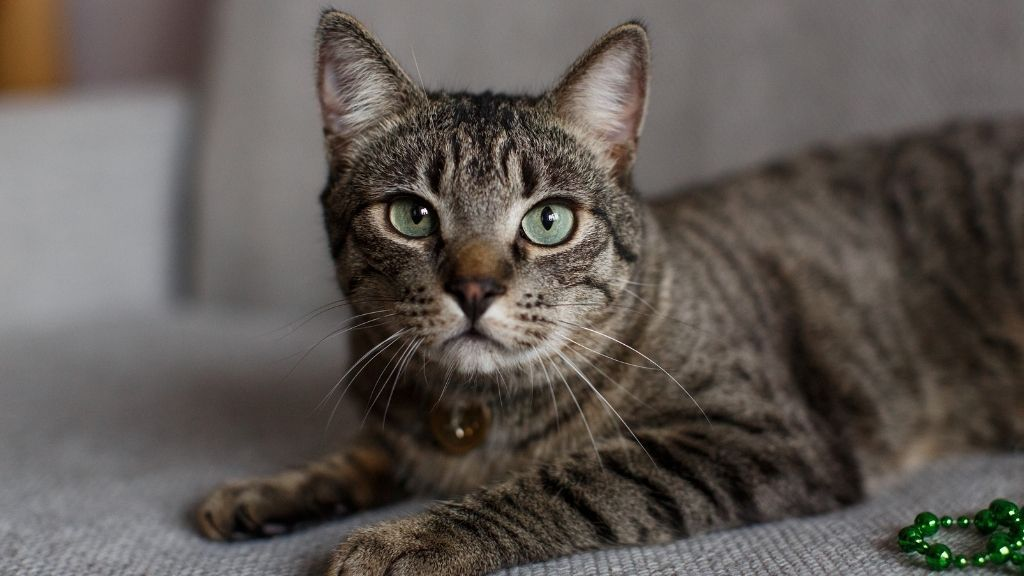
\includegraphics[width=0.7\textwidth]{cat.jpg}| \par
\verb|    \caption{Figure caption.}| \par
\verb|    \label{fig:label1} %Use this to reference the figures in the text| \par
\verb|\end{figure}| \par
\noindent
This code creates Figure \ref{fig:my_label}. \par
\begin{figure}[h]
    \centering
    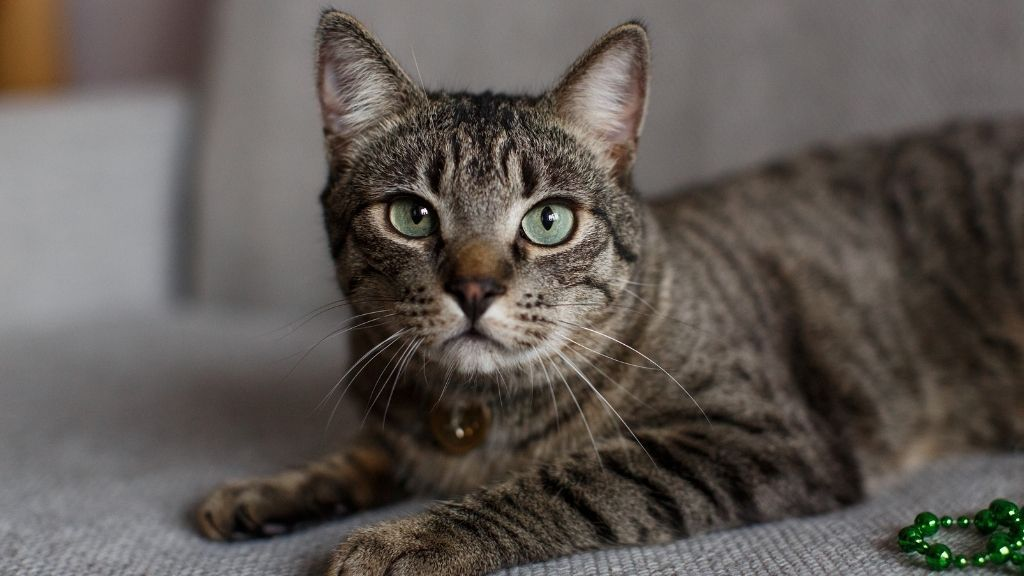
\includegraphics[width=0.7\textwidth]{cat.jpg}
    \caption{Figure caption.}
    \label{fig:my_label} %Change font settings
\end{figure}
%\noindent
And you can reference it in the text with \verb|\ref{label}|, replacing \verb|label| with the figure label (\verb|fig:label1| in this example).  

\subsection{Tables}
\noindent
To add tables you can use the \textbf{table} environment. An example is \par
\verb|\begin{table}[h]| \par
\verb|    \centering| \par
\verb|    \caption{Table caption.}| \par
\hskip 0.8cm\EscVerb{\\begin\{tabular\}\{l|c||r\}} \par
\verb|        \thickline| \par
\verb|        \textbf{Left aligned} & \textbf{Centered} & \textbf{Right aligned} \\| \par
\verb|        \thickline %Make it bold/thicker| \par
\verb|        a & b & c \\| \par
\verb|        \hline| \par
\verb|        d & e & f \\| \par
\verb|        \hline| \par
\verb|        \hline| \par
\verb|        g & h & i \\| \par
\verb|        \thicklinec{0.4}{0.2} %use this to make a custom thick line| \par
\verb|    \end{tabular}| \par
\verb|    \label{tab:label1}| \par
\verb|\end{table}| \par
\noindent
This code creates Table \ref{tab:my_label}. \par
\begin{table}[h]
    \centering
    \caption{Table caption.}
    \begin{tabular}{l|c||r}
        \thickline
        \textbf{Left aligned} & \textbf{Centered} & \textbf{Right aligned} \\
        \thickline %Make it bold/thicker
        a & b & c \\
        \hline 
        d & e & f \\
        \hline
        \hline
        g & h & i \\
        \thicklinec{0.4}{0.2} %use this to make a thick line
    \end{tabular}
    \label{tab:my_label}
\end{table}
%\noindent
And you can reference it the same way as you would reference figures. Make sure the caption goes before the tabular environment, because the House Style says table captions must go on top of the table.

\newpage
\subsection{Maths}
\noindent
To add equations you can use the \textbf{texteqn} and \textbf{nonumtexteqn} environments. The \textbf{nonumtexteqn} creates equations that are not numbered. Sometimes using \verb|\frac{}{}| creates very small text that is difficult to read, use \verb|\ddfrac{}{}| instead. Using \verb|\frac{}{}|
\begin{texteqn}
$\frac{dy}{dx} = nx^{n-1}$
\label{eqn:1}
\end{texteqn}
Using \verb|\ddfrac{}{}|
\begin{texteqn}
$\ddfrac{dy}{dx} = nx^{n-1}$
\label{eqn:2}
\end{texteqn}
You can also add \verb|\label{}| inside both environments to be able to reference the mathematical expressions in the text. \par
When you are writing quantities with units and you do not want that they get separated in two different lines you can use the command \verb|\data{}|.

\subsection{Lists}
\noindent
Lists must be numbered so use the \textbf{numlist} environment.

\section{Extra stuff}
\noindent
Some commands and environments that I have added just for fun and are hopefully useful to some people.

\begin{boxed}{Box title}
\textbf{boxed} environment, which takes a parameter to set the box title. This parameter can just be left empty to not set any title to the box. This environment may be useful to highlight important definitions or equations. \par
%\begin{center}
    \hfill\verb|\begin{boxed}{Box title} ... \end{boxed}|
%\end{center}
\end{boxed}

\noindent
I have also added the \verb|\makecoverpage| command. It makes a cover page that includes the title, subtitle, university, department, country, author and date. When calling this command the page numbering starts from page 2 (counting from 1) and the page number is on the top right in all pages. \par
To set the subtitle, university, department and country you can use the commands \par
\verb|\setsubtitle{}| \par
\verb|\setuniversity{}| \par
\verb|\setdepartment{}| \par
\verb|\setcountry{}| \par
\noindent
You have to call these commands before making the cover page or the changes will not apply. Figure \ref{fig:cover} shows how the cover page looks.

\begin{figure}[h]
    \centering
    
\includegraphics[width=0.6\textwidth]{coverpage.png}
    \caption{Cover page.}
    \label{fig:cover}
\end{figure}

\addcontentsline{toc}{section}{References}
\printbibliography
\end{document}
